\chapter{Metodología}

\section{Preprocesamiento de imágenes}
\subsection{Normalización del fondo}
Variaciones en el color del fondo pueden afectar la capacidad del modelo para aprender características relevantes, desviando su atención hacia patrones irrelevantes. Por ello, se aplica un proceso de normalización del fondo, asegurando que la información procesada esté centrada en la región de interés y no en elementos circunstanciales de la adquisición de la imagen.
En primer lugar, la imagen original se convierte a escala de grises utilizando la transformación de OpenCV\footnote{OpenCV. (s.f.). Open Source Computer Vision Library. OpenCV Documentation. \url{https://docs.opencv.org/}}:

\[
RGB[A] \;to \;Gray: Y \leftarrow 0.299 \cdot R \;+\; 0.587 \cdot G \;+\; 0.114 \cdot B
\]

donde R,G,B son los valores de los canales rojo, verde y azul respectivamente.
Luego, se calcula la distribución de intensidades mediante un conteo de frecuencias de los valores de píxeles. Si la intensidad con mayor frecuencia corresponde a 255, se infiere que el fondo de la imagen es blanco. En este caso, todos los píxeles con valor 255 en la imagen original son reemplazados por 0 (negro). En caso contrario, la imagen se mantiene sin modificaciones.

\begin{center}
	\begin{figure}[H]
		\centering
		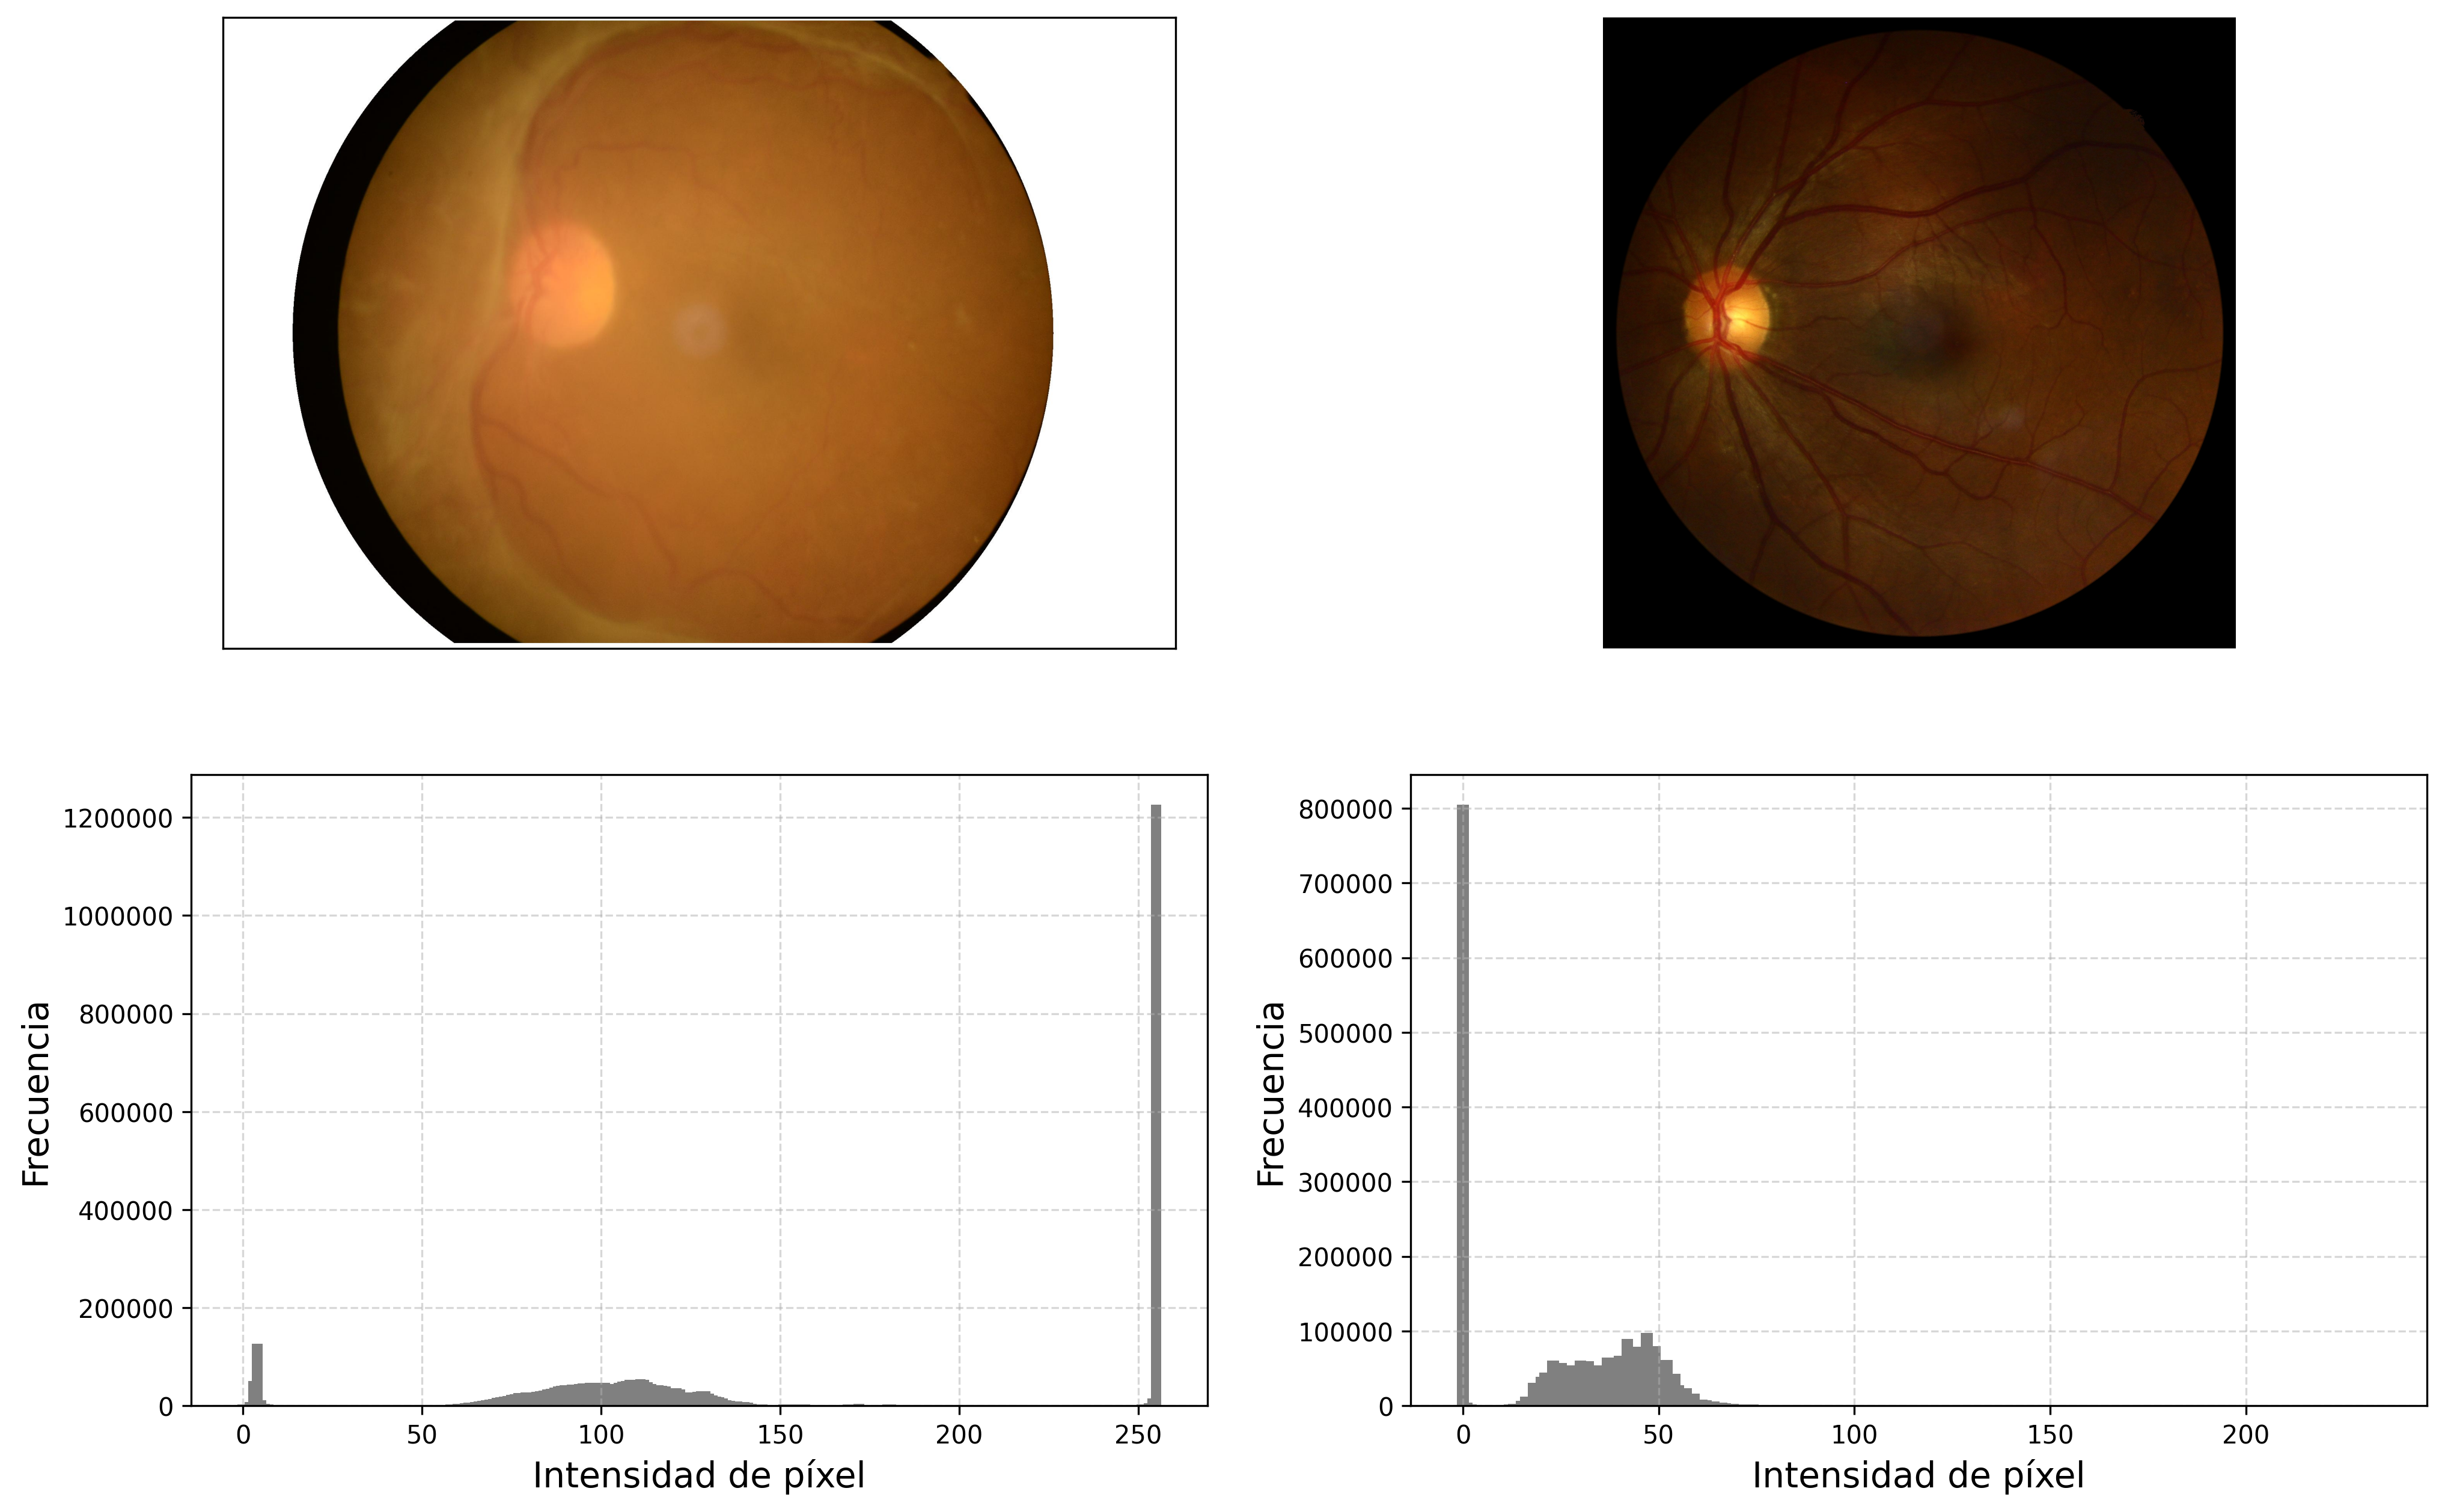
\includegraphics[scale=0.40]{doc_images/histograma_con_imagenes.png}
		\caption{Comparación de dos imágenes de fondo de ojo (izquierda: fondo blanco, derecha: fondo negro) y sus respectivos histogramas de intensidad en escala de grises.} 
		\label{fig:histograma_con_imagenes}
	\end{figure}
\end{center}

\begin{center}
	\begin{figure}[H]
		\centering
		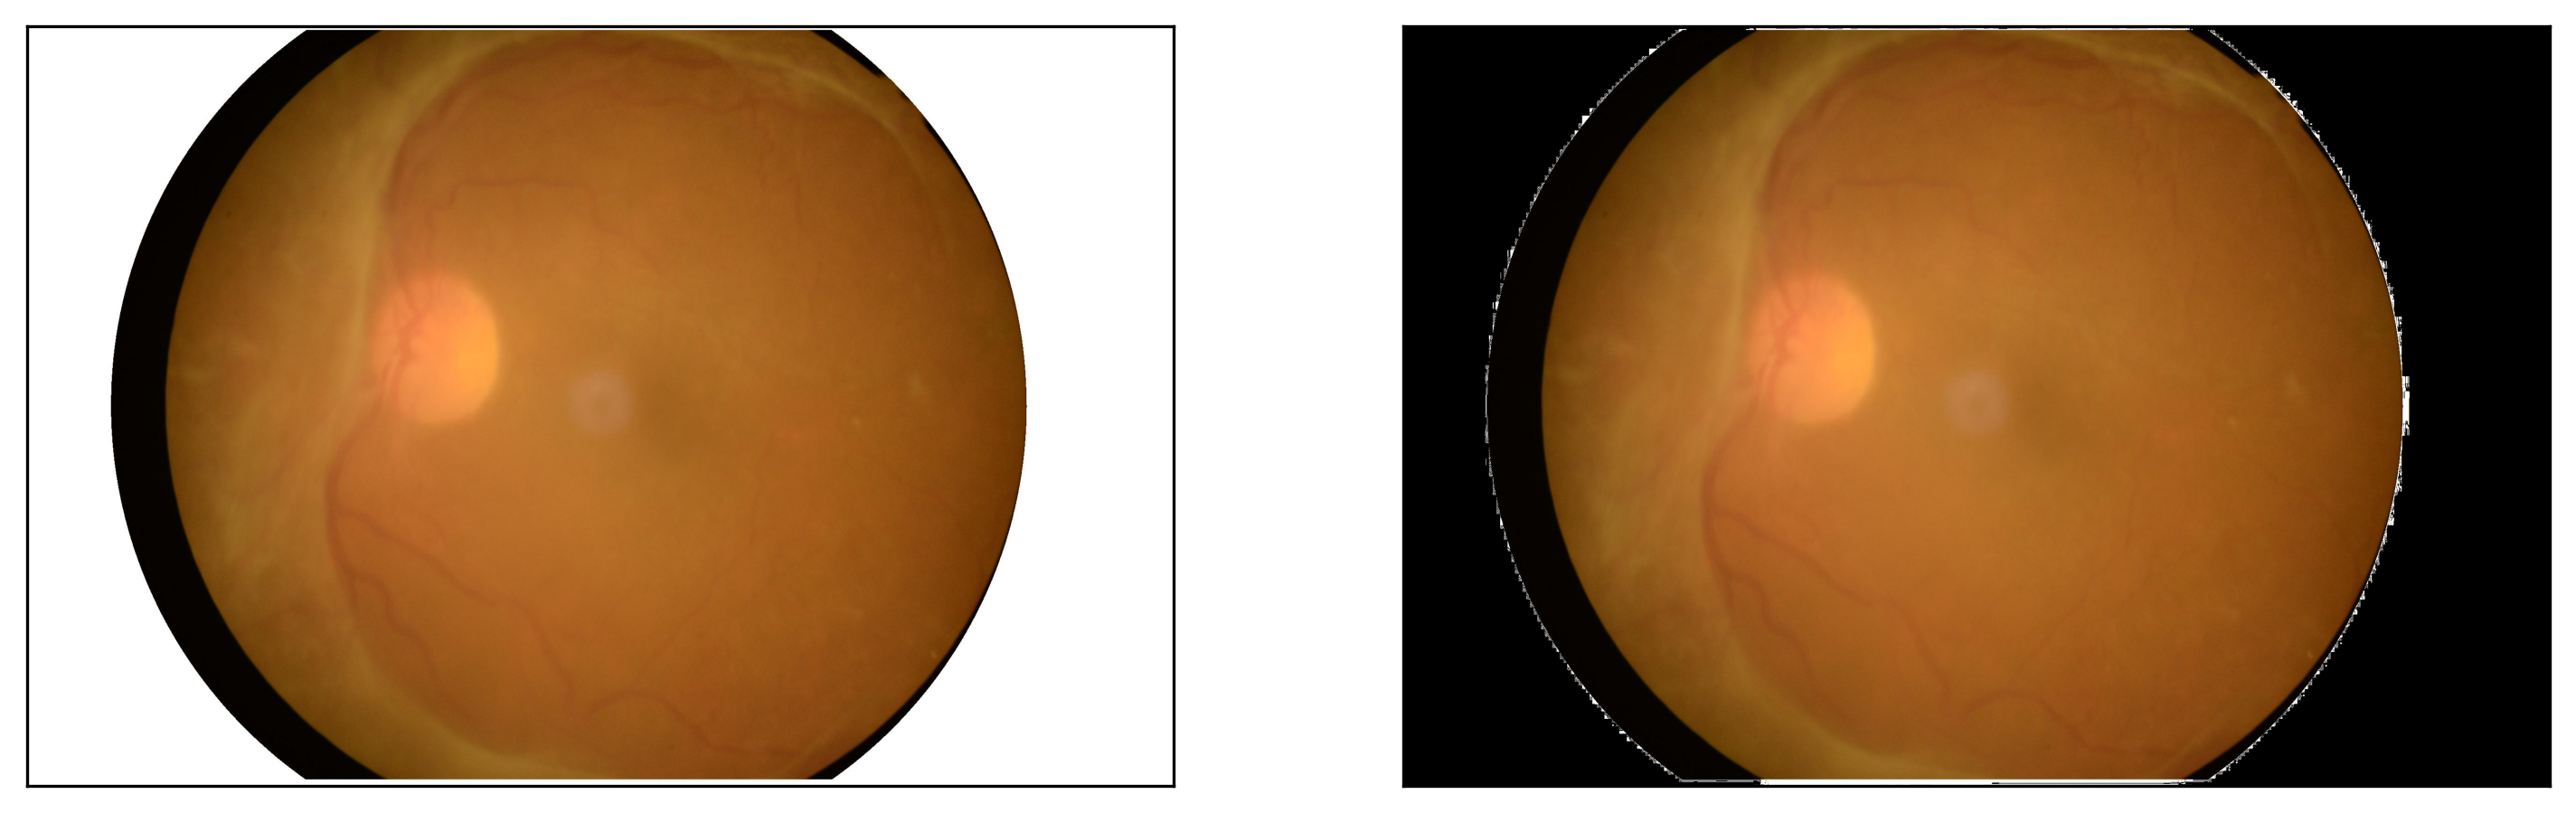
\includegraphics[scale=0.60]{doc_images/fondo_blanco_a_negro.png}
		\caption{Imagen original (izquierda) y versión modificada (derecha), donde los píxeles de fondo blanco (valor 255) fueron reemplazados por negro (valor 0).} 
		\label{fig:fondo_blanco_a_negro}
	\end{figure}
\end{center}

\subsection{FOV (Field of View)}
Dado que la región de interés en estas imágenes presenta una forma circular bien definida, se emplea un método basado en la detección de círculos para segmentar el campo de visión (FOV) en la imagen de fondo de ojo.

Inicialmente, la imagen se convierte a escala de grises y se aplica un filtro de desenfoque de mediana\footnote{Filtro de desenfoque de mediana: técnica digital que se usa para reducir el ruido en imágenes, videos y señales, preservando bordes y esquinas redondeadas.} para reducir el ruido sin perder bordes significativos. Luego, se intenta detectar un círculo en la imagen mediante la transformada de Hough\footnote{La transformada de Hough busca estructuras circulares en imágenes en escala de grises al analizar bordes y acumular votos en un espacio de parámetros, lo que permite identificar círculos de diferentes tamaños.} para círculos, utilizando la función cv2.HoughCircles de OpenCV con la siguiente configuración:

\begin{itemize}
	\item minDist = cols // 2: Establece la distancia mínima entre los centros de los círculos detectados. Dado que se busca un único círculo, se asigna un valor alto para evitar detectar múltiples círculos superpuestos.
	\item param1 = 60: Define el umbral superior del detector de bordes de Canny\footnote{El detector de bordes de Canny es un algoritmo que identifica bordes en una imagen aplicando un filtro gaussiano para suavizar el ruido, calculando el gradiente de intensidad y utilizando dos umbrales para eliminar bordes débiles y mantener solo los más relevantes.}. Valores bajos detecta más bordes mientras que un valor más alto detecta solo los bordes fuertes, reduciendo el ruido en la detección.
	\item{param2 = 30: Es el umbral del acumulador de Hough. Valores bajos pueden generar más falsos positivos, mientras que valores altos aseguran que solo se detecten círculos bien definidos.}
	\item{minRadius = min(rows, cols) // 4 y maxRadius = max(rows, cols) // 2: Se establecen estos valores para garantizar que el círculo detectado abarque la mayor parte de la imagen, ya que en las imágenes de fondo de ojo el área de interés generalmente ocupa una gran proporción del total.}
\end{itemize}

Si se detecta un único círculo, se genera una máscara binaria del mismo tamaño que la imagen, donde se marca con intensidad 255 (blanco) el área correspondiente al círculo identificado como la región del FOV.

\begin{center}
	\begin{figure}[H]
		\centering
		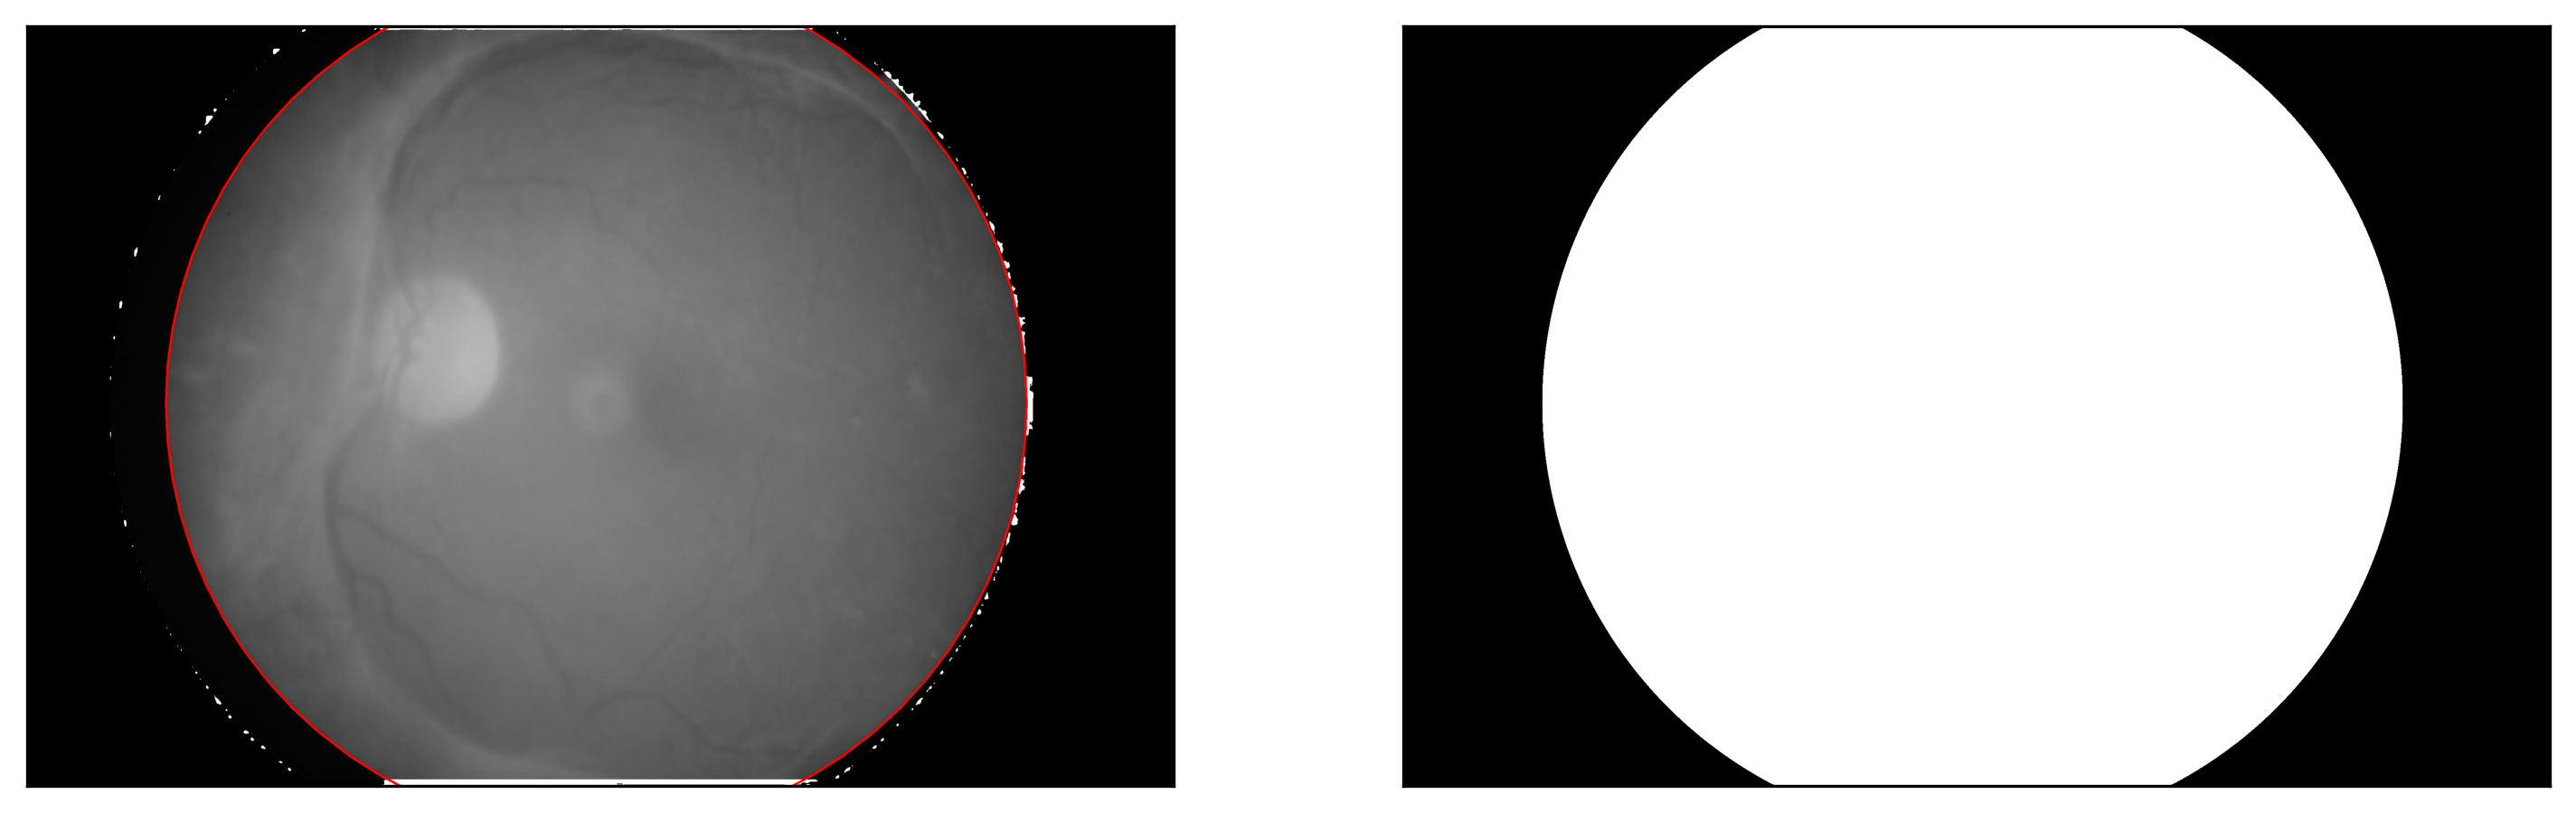
\includegraphics[scale=0.60]{doc_images/circulos_hough.png}
		\caption{A la izquierda, imagen con desenfoque de mediana y círculo detectado (en rojo) mediante la transformada de Hough. A la derecha, máscara binaria generada a partir del círculo.} 
		\label{fig:circulos_hough}
	\end{figure}
\end{center}

Si el método basado en la transformada de Hough no detecta ningún círculo o detecta más de uno, se recurre a un enfoque alternativo basado en la suma de intensidades de los canales de la imagen. Las imágenes de fondo de ojo son a color, por lo que están compuestas por tres canales (rojo, verde y azul), cada uno con valores de intensidad entre 0 (negro) y 255 (blanco). Al sumar las intensidades de los tres canales en cada píxel, se obtiene una imagen en escala de grises que acentúa las diferencias entre las regiones con contenido retiniano (dentro del FOV) y el fondo. Esto resulta útil en casos donde el fondo no es completamente negro, como ocurre con ciertas cámaras que introducen ruido o iluminaciones residuales. De este modo, se mejora el contraste entre el FOV y el resto de la imagen.

Luego, se aplica el umbral de Otsu para determinar un valor de corte que permita separar ambas regiones. Este método analiza el histograma de intensidades de la imagen y selecciona automáticamente un valor de umbral que minimiza la varianza dentro de cada clase y maximiza la varianza entre clases, separando así de forma óptima los píxeles en dos grupos: uno que representa los objetos (en este caso, la retina) y otro el fondo. Se genera una máscara binaria donde los píxeles con valores superiores al umbral se asignan como \textit{True} y el resto como \textit{False}. Finalmente, se realiza un relleno de agujeros\footnote{Para realizar el relleno de agujeros se utiliza la función \textit{binary\_fill\_holes} del módulo ndimage de SciPy. Esta función identifica regiones cerradas dentro de los objetos binarios (representadas por \textit{False} rodeados de \textit{True}) y las completa.} sobre la máscara binaria, garantizando que la región segmentada sea continua y sin interrupciones.

\begin{center}
	\begin{figure}[H]
		\centering
		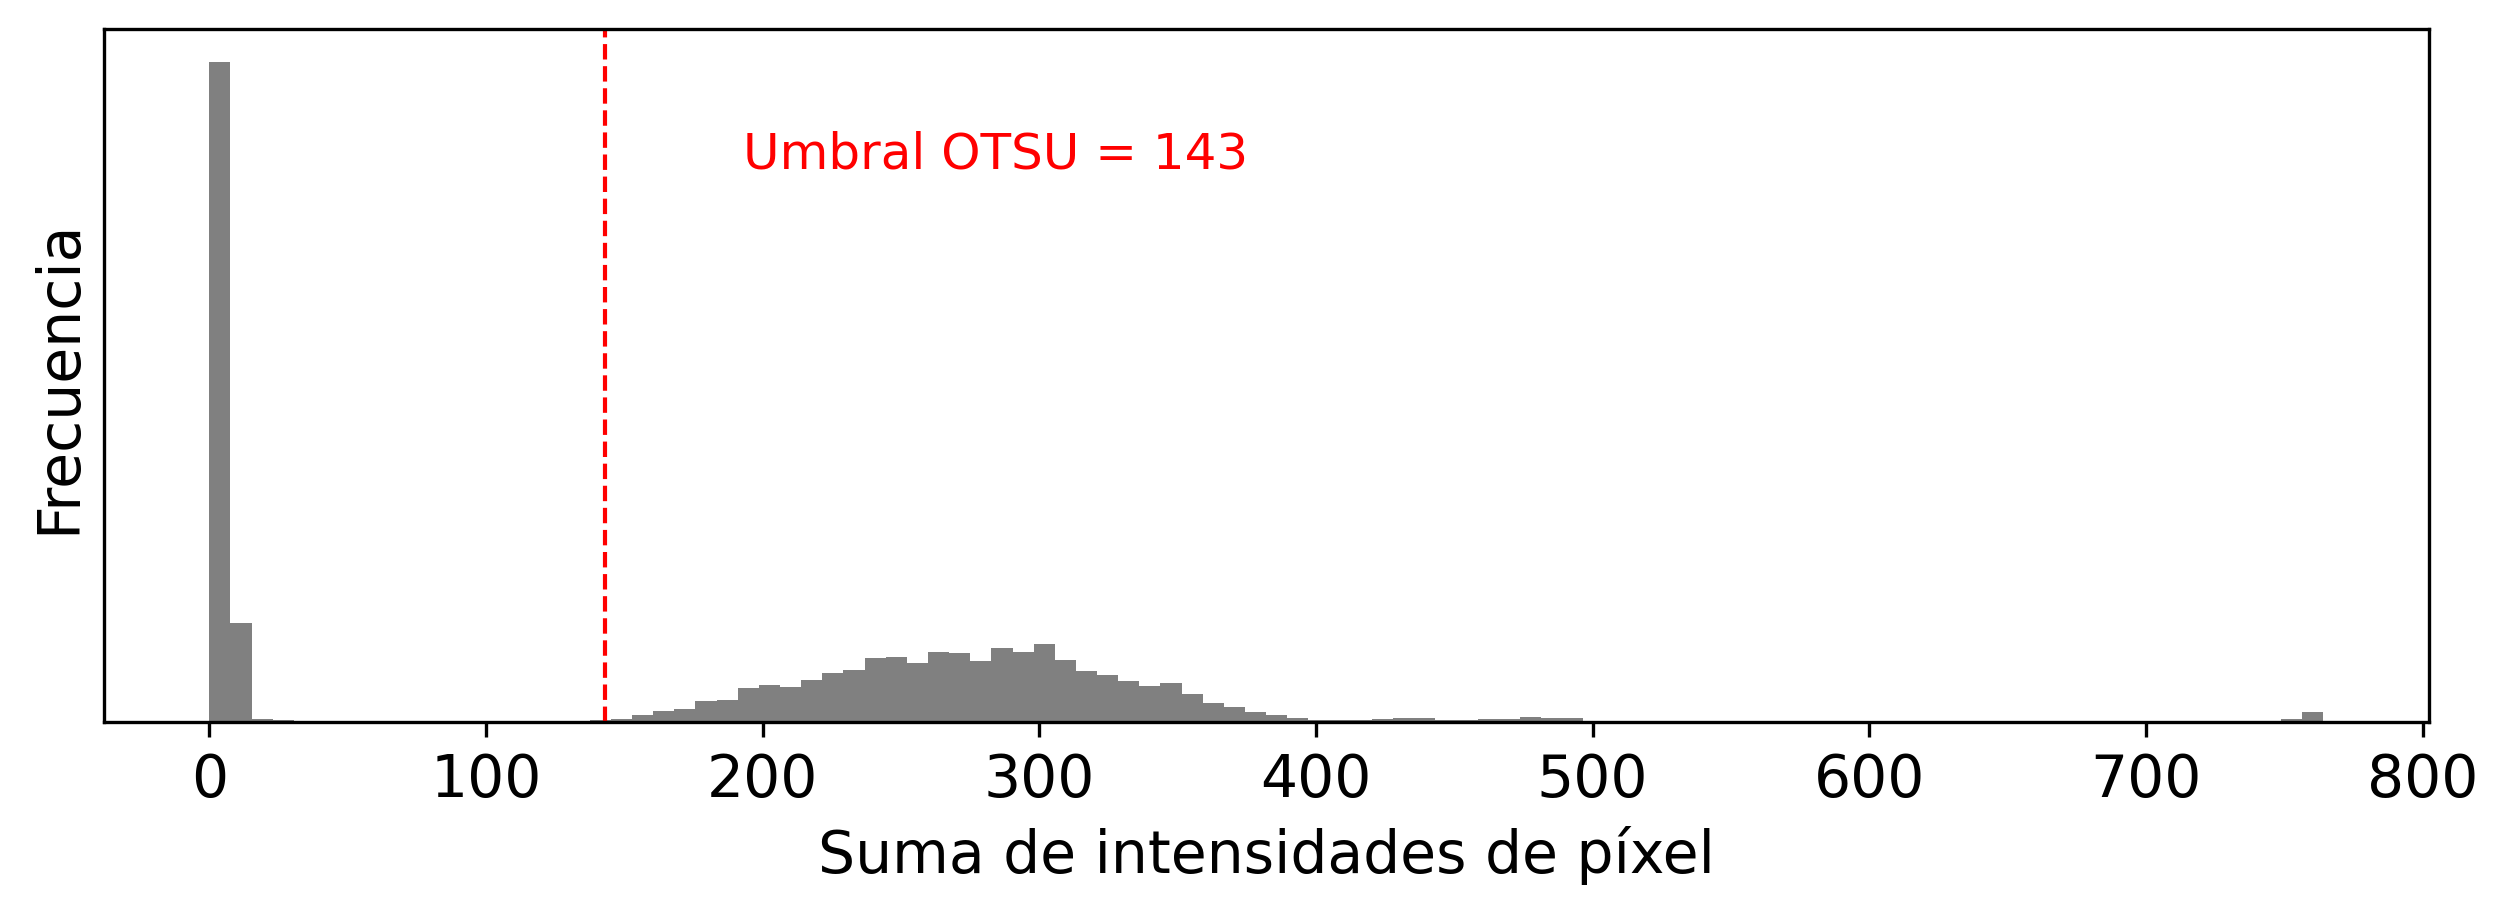
\includegraphics[scale=0.60]{doc_images/histograma_suma.png}
		\caption{Histograma de la suma de intensidades RGB en imágenes donde la transformada de Hough no detectó un único círculo.} 
		\label{fig:histograma_suma}
	\end{figure}
\end{center}

\subsection{Ajuste del tamaño de la imagen}
Una vez obtenida la máscara del campo de visión (FOV), se aplica una función que permite recortar la imagen original, conservando únicamente la región correspondiente al contenido retiniano. En primer lugar, se utiliza la máscara para establecer en negro (intensidad cero) todos los píxeles de la imagen que se encuentran fuera del área delimitada como FOV, eliminando así cualquier información irrelevante o artefactos. Luego, se identifican las coordenadas de un rectángulo (bounding box) que encierra completamente la región marcada como FOV en la máscara binaria. Finalmente, se recorta la imagen utilizando dichas coordenadas, devolviendo únicamente la porción útil.

\subsection{Recorte del Bounding Box}
Para finalizar el preprocesamiento, la imagen segmentada y recortada se redimensiona a un tamaño fijo de 512×512 píxeles\footnote{En este caso se elige un tamaño de 512×512 píxeles, que permite preservar mayor detalle que resoluciones más bajas, sin comprometer demasiado el rendimiento computacional.}. Aunque arquitecturas como ResNet permiten procesar imágenes de distintas dimensiones gracias al uso de adaptive pooling, establecer una resolución estándar facilita el procesamiento en lotes y permite un uso más eficiente de los recursos computacionales.

\section{Normalización de imágenes}
Una vez redimensionadas, se calcula la media y el desvío estándar de los valores de píxel por canal (R, G, B) en el conjunto de entrenamiento. En este caso, los valores obtenidos fueron:

\begin{itemize}
	\item \textbf{Media}: [0.1948, 0.2880, 0.4238]
	\item \textbf{Desvío estandar}: [0.1661, 0.2021, 0.2782]
\end{itemize}

Estos valores se utilizan para normalizar las imágenes, es decir, restar la media y dividir por el desvío en cada canal.

Esta técnica ayuda a estabilizar el entrenamiento: Al quedar los valores normalizados en un rango cercano a -1 y 1, las actualizaciones de los pesos se vuelven más uniformes, evitando saltos muy grandes o avances demasiado pequeños durante la optimización. Además, valores de entrada en escalas similares permiten que el algoritmo de optimización (como el gradiente descendente) converja más rápido, ya que las actualizaciones de los parámetros no se ven afectadas por magnitudes desiguales. Como beneficio adicional, la normalización reduce el riesgo de que ciertas regiones con valores más altos dominen sobre otras, lo que puede dificultar que el modelo aprenda representaciones relevantes. 

\subsection{Data Augmentation}
Antes de entrenar el modelo, se aplican técnicas de data augmentation al conjunto de entrenamiento. Estas técnicas introducen variaciones artificiales en las imágenes (como rotaciones, recortes aleatorios o volteos horizontales), con el objetivo de aumentar la diversidad de los datos y evitar que memorice patrones específicos de los datos de entrenamiento.
En este trabajo se utilizaron tres transformaciones principales sobre las imágenes de entrenamiento:

\begin{itemize}
	\item Volteo horizontal aleatorio (RandomHorizontalFlip): con una probabilidad del 50\%, la imagen se invierte de izquierda a derecha.
	\item Rotación aleatoria (RandomRotation): rota la imagen un ángulo aleatorio entre -15° y 15°, utilizando interpolación bilineal para preservar la calidad de la imagen y rellenando las zonas vacías con negro.
	\item{Volteo vertical aleatorio (RandomVerticalFlip): con una probabilidad del 50\%, la imagen se invierte de arriba hacia abajo.}
\end{itemize}

Es importante destacar que en las imágenes de fondo de ojo no siempre se sigue una orientación estándar: pueden estar centradas en la mácula, en el disco óptico o presentar leves inclinaciones según cómo se haya realizado la captura. Por eso, introducir variaciones como rotaciones y volteos durante el entrenamiento ayuda al modelo a enfocarse en las características relevantes de la imagen, sin depender de la posición exacta de las estructuras anatómicas.

\subsection{Arquitectura}
En este trabajo se utilizó una arquitectura basada en ResNet-18, una red convolucional profunda con conexiones residuales que permiten un entrenamiento más eficiente y estable. La ResNet-18 se compone de bloques residuales que aprenden ajustes sobre la representación existente en lugar de reemplazarla por completo, lo que facilita el flujo de gradientes y evita problemas comunes en redes profundas, como la degradación del rendimiento al aumentar la cantidad de capas.

\begin{center}
	\begin{figure}[H]
		\centering
		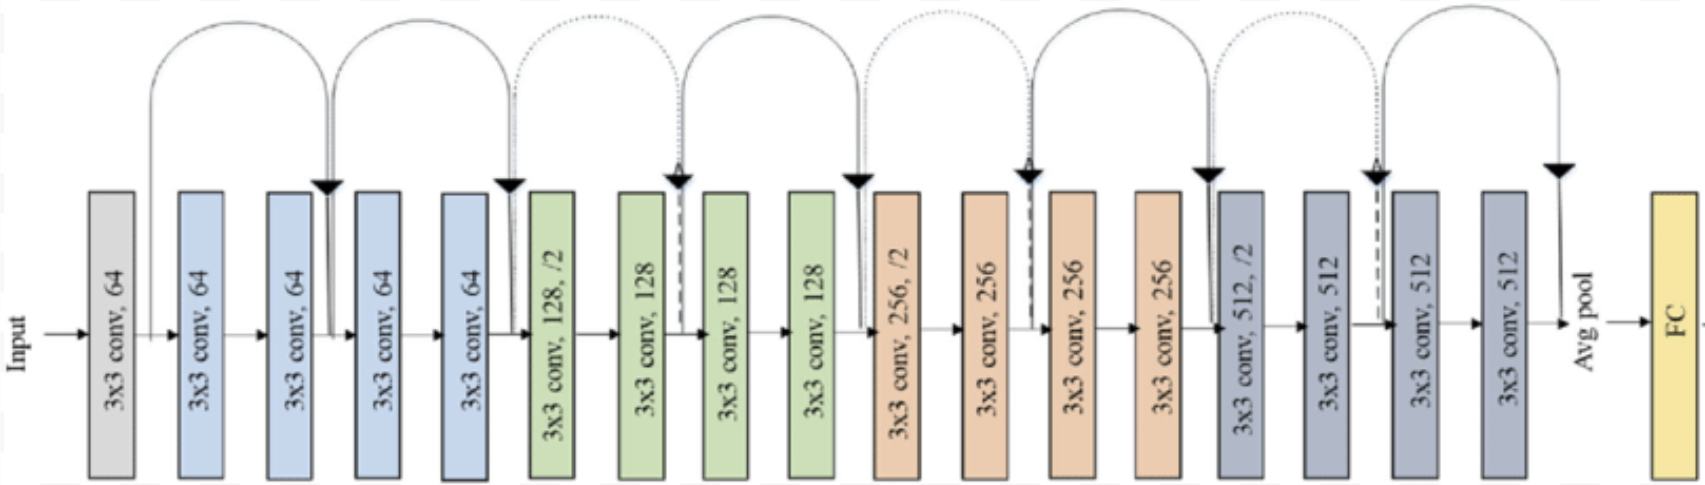
\includegraphics[scale=0.70]{doc_images/resnet18.png}
		\caption{Arquitectura de la red ResNet-18.} 
		\label{fig:resnet18}
	\end{figure}
\end{center}

La arquitectura de ResNet-18 se compone de una capa convolucional inicial, seguida por cuatro etapas residuales compuestas por bloques básicos (BasicBlocks), y una capa final de clasificación. El cuadro \ref{tab:resnet18} resume las principales características de cada etapa de la red.


\begin{table}[H]
	\centering
	\renewcommand{\arraystretch}{1.5}
	\resizebox{\textwidth}{!}{
		\begin{tabular}{ ||c|c||  }
			\hline
			\hline
			\textbf{Etapa} & \textbf{Descripción} \\
			\hline
			\hline
			\cellcolor[HTML]{d6d1d1} \textbf{Capa Inicial} & 
			\makecell[l]{- Conv2d (7×7, stride 2, padding 3)\\
				- BatchNorm \\
				- ReLU \\
				- MaxPooling (3x3, stride 2)} \\		
			\hline
			\hline
			\cellcolor[HTML]{abd6f7} \textbf{Etapa residual 1} & - 2 x BasicBlock con 64 filtros, stride 1 \\		
			\hline
			\hline
			\cellcolor[HTML]{a9dda2} \textbf{Etapa residual 2} & - 2 x BasicBlock con 128 filtros, el primero con stride 2 \\		
			\hline
			\hline
			\cellcolor[HTML]{ffb980} \textbf{Etapa residual 3} & - 2 x BasicBlock con 256 filtros, el primero con stride 2 \\		
			\hline
			\hline
			\cellcolor[HTML]{9ab2c1} \textbf{Etapa residual 4} & - 2 x BasicBlock con 512 filtros, el primero con stride 2 \\		
			\hline
			\hline
			\cellcolor[HTML]{fbdc89} \textbf{Capa Final} & 
			\makecell[l]{- Global Average Pooling \\
				- Capa totalmente conectada (2 salidas: buena o mala calidad)} \\
			\hline
		\end{tabular}
	}
	\caption{Componentes principales de la arquitectura ResNet-18.}
	\label{tab:resnet18}
\end{table}


Cada una de las etapas residuales mencionadas se compone de dos BasicBlocks, cuya estructura se detalla a continuación:
\begin{itemize}
	\item Conv2d (3x3)
	\item BatchNorm
	\item ReLU
	\item Conv2d (3x3)
	\item BatchNorm
	\item Suma residual: \textit{F(x) + x}
\end{itemize}

\begin{center}
	\begin{figure}[H]
		\centering
		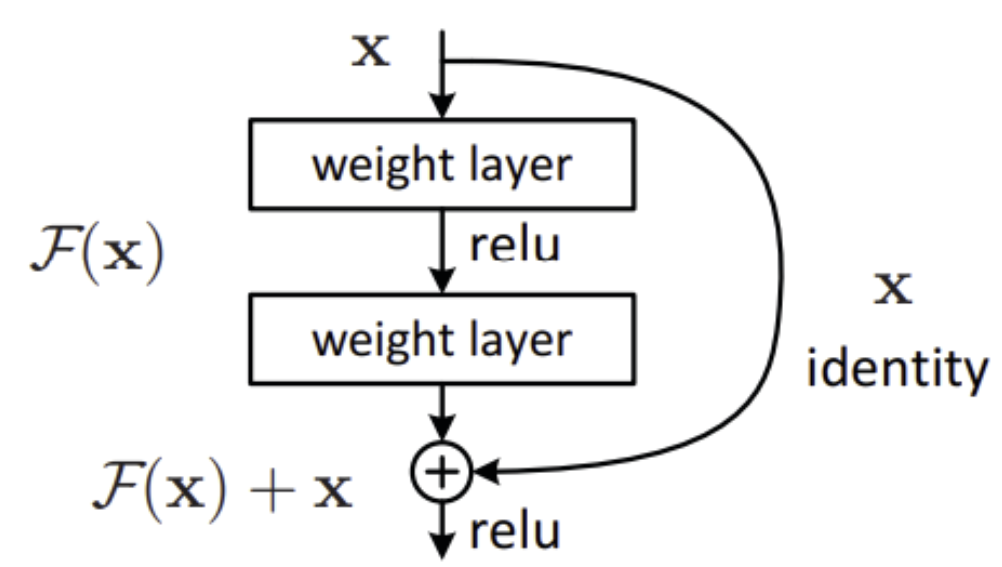
\includegraphics[scale=0.70]{doc_images/residual.png}
		\caption{Estructura de un bloque residual (BasicBlock). La entrada “x” se bifurca en dos caminos: uno donde se aplican dos capas convolucionales y otro que preserva la señal original con una conexión identidad. Finalmente, ambas salidas se suman y se aplica una función de activación ReLU \parencites{he2015deep}.} 
		\label{fig:residual}
	\end{figure}
\end{center}

En una red sin conexiones residuales, cada capa debe aprender directamente la transformación completa que mapea una entrada a una salida deseada. Esto implica que, si una capa no logra detectar patrones relevantes, por ejemplo, si una capa intermedia genera activaciones nulas o muy bajas, las siguientes capas se ven forzadas a operar sobre representaciones poco informativas, comprometiendo la capacidad de aprendizaje del modelo. Además, a medida que aumenta la profundidad de la red, puede intensificarse el problema del desvanecimiento del gradiente\footnote{El desvanecimiento del gradiente es un problema que ocurre en redes neuronales profundas cuando los gradientes que se propagan hacia las capas iniciales se vuelven extremadamente pequeños. Durante la retropropagación del error, los gradientes se multiplican sucesivamente mediante la regla de la cadena. Si las derivadas de las funciones de activación son pequeñas, esto provoca que los gradientes se reduzcan exponencialmente a medida que se avanza hacia las capas cercanas a la entrada, impidiendo que reciban actualizaciones significativas y dificultando el entrenamiento de la red.}, dificultando la retropropagación efectiva del error hacia las capas iniciales.

Las conexiones residuales mitigan ambos problemas: facilitan la propagación directa de la información útil a través de la red y simplifican la optimización, ya que el modelo aprende únicamente la diferencia entre la entrada y la salida deseada. Esto mejora tanto la precisión como la eficiencia del entrenamiento.

La arquitectura ResNet-18 fue seleccionada por ser una de las más utilizadas en investigaciones de visión computacional, especialmente en contextos de transferencia de aprendizaje. Su popularidad se debe a una combinación de factores: ofrece una buena capacidad de representación con una profundidad moderada que facilita el entrenamiento, es robusta frente a distintas tareas, y puede adaptarse a imágenes de entrada de diferentes tamaños sin requerir preprocesamiento estricto. Además, su disponibilidad como modelo preentrenado en conjuntos de datos grandes como ImageNet permite reutilizar conocimientos previamente aprendidos y adaptarlos eficazmente a nuevos dominios con datos limitados, como en el caso de este trabajo. Diversos estudios han demostrado que ResNet-18 puede lograr buenos resultados en aplicaciones médicas específicas, incluso cuando se dispone de un conjunto de datos reducido \parencites{kim2022transfer}.


\section{Entrenamiento utilizando transfer learning}
En la práctica, entrenar una red convolucional desde cero no es habitual, ya que esto requiere conjuntos de datos muy grandes para lograr un buen resultado. Por este motivo, una estrategia común consiste en utilizar redes previamente entrenadas en bases de datos extensas, como ImageNet, que contiene más de un millón de imágenes clasificadas en mil categorías. Esta estrategia, conocida como transfer learning, permite aprovechar los conocimientos adquiridos por la red en tareas generales y adaptarlos a un nuevo problema con menos datos disponibles. Existen dos enfoques principales: el uso de la red como extractor de características (feature extraction), donde se aprovechan las representaciones internas aprendidas sin modificar sus pesos, y el fine-tuning, que implica ajustar los pesos de la red preentrenada, total o parcialmente, en función del nuevo conjunto de datos \parencites{cs231n2023transfer}. Como señala \cite{stevens2020deep}, esta última estrategia combina lo mejor de dos mundos: reutiliza características previamente aprendidas por otra red en una tarea diferente (en lugar de diseñarlas manualmente, como se hacía antes del aprendizaje profundo), y al mismo tiempo permite adaptarlas a las particularidades del nuevo problema mediante entrenamiento adicional.

En este trabajo se utilizó una estrategia de fine-tuning a partir de una red ResNet-18 preentrenada en ImageNet. Inicialmente, se reemplazó la capa de clasificación original de la red por una nueva capa adaptada a la tarea específica de clasificación de calidad de imagen. En una primera etapa, se entrenó únicamente esta nueva capa, manteniendo congelados los pesos del resto de la red. Luego, se descongelaron las capas más profundas para continuar el entrenamiento y permitir que el modelo ajustara parcialmente sus representaciones a las características propias del nuevo dominio. Esta decisión se basa en la noción de que las primeras capas de una red convolucional suelen capturar características visuales de bajo nivel, como bordes, texturas y formas simples, que tienden a ser comunes a una gran variedad de imágenes \parencites{stevens2020deep}. Por lo tanto, mantenerlas congeladas ayuda a preservar ese conocimiento general y reduce el riesgo de sobreajuste.

Las estrategias exploradas incluyeron desde el entrenamiento exclusivo de la capa final, manteniendo congeladas el resto de las capas, hasta el fine-tuning progresivo de bloques más profundos de la red, con el objetivo de evaluar el impacto de permitir el ajuste de representaciones internas más complejas. En todos los casos, se utilizaron técnicas estándar de entrenamiento tales como el uso de data augmentation, optimización con Stochastic Gradient Descent (SGD) o Adam (Adaptive Moment Estimation), programación del learning rate mediante scheduler, y entrenamiento con precisión mixta (Automatic Mixed Precision, AMP\footnote{Automatic Mixed Precision: método de Pytorch que permite usar dos tipos de precisión, float16 solo en operaciones que no necesitan tanta precisión, como multiplicaciones de matrices, mientras que,
	algunas operaciones críticas (como la suma de gradientes) siguen en float32 para evitar errores numéricos. \url{https://pytorch.org/tutorials/recipes/recipes/amp_recipe.html}}) para optimizar el uso de la GPU y un tamaño de batch de 128.
	
Las figuras \ref{fig:filtrosConv1}, \ref{fig:actConv1}, \ref{fig:actLayer1}, \ref{fig:actLayer2}, \ref{fig:actLayer3}, \ref{fig:actLayer4} del anexo muestran las características de bajo nivel capturadas por la capa inicial de la ResNet-18 (filtros de bordes y texturas) y el comportamiento interno de sus capas más profundas (mapas de activación de cada bloque).

\section{Función de pérdida}
Para la tarea de clasificación binaria se utilizó la función de pérdida de entropía cruzada (Cross Entropy Loss\footnote{\url{https://pytorch.org/docs/stable/generated/torch.nn.CrossEntropyLoss.html}}), ampliamente empleada en problemas de clasificación supervisada. Esta función mide la discrepancia entre la distribución de probabilidad predicha por el modelo y la verdadera etiqueta de clase, penalizando con mayor severidad aquellas predicciones erróneas en las que el modelo está muy confiado. Cuando el modelo asigna una probabilidad alta a la clase equivocada, el logaritmo de dicha probabilidad es cercano a cero y su negativo produce un valor alto, lo que se traduce en una penalización significativa. Por el contrario, si la probabilidad de la clase equivocada es baja, la penalización será menor. Gracias a esto, el modelo aprende a no “confiar ciegamente” en predicciones incorrectas.

\section{Optimizadores}
Durante el entrenamiento de una red neuronal, el objetivo es encontrar los valores óptimos de los pesos que minimicen una función de pérdida. Para ello, se utilizan algoritmos de optimización basados en el cálculo del gradiente, que actualizan los pesos del modelo en función del error cometido. El más utilizado de estos algoritmos es el descenso del gradiente (GD).

El descenso del gradiente es un método iterativo que busca minimizar una función de pérdida calculando las derivadas parciales de dicha función con respecto a cada uno de los parámetros del modelo. Este conjunto de derivadas forma el gradiente e indica la dirección en la que la función crece más rápidamente. Por lo tanto, la actualización de los pesos se realiza en la dirección contraria, es decir, hacia el mínimo. La magnitud del paso de actualización está determinada por un hiperparámetro conocido como tasa de aprendizaje (learning rate).

La actualización de cada parámetro  se realiza según la siguiente regla:

\[
\Delta w \;=\; -\,\eta\,\frac{\partial L}{\partial w} \quad\Longrightarrow\quad
w \leftarrow w + \Delta w
\]

donde:
\begin{itemize}
	\item $\Delta w$ w es el cambio aplicado al parámetro.
	\item $\eta$ es la tasa de aprendizaje.
	\item $\frac{\partial L}{\partial w}$ es la derivada parcial de la función de pérdida respecto a $w$.
\end{itemize}

El método clásico de descenso del gradiente se calcula utilizando todos los ejemplos del conjunto de entrenamiento, lo cual resulta computacionalmente costoso y lento, especialmente con grandes volúmenes de datos. En este trabajo se utilizó una variante de este método, el Stochastic Gradient Descent (SGD), que actualiza los pesos del modelo utilizando pequeños lotes de datos (mini-batches) en lugar de todo el conjunto de entrenamiento. Este enfoque, aunque introduce ciertas aproximaciones imprecisas, favorece la convergencia del modelo y evita que el proceso de optimización se quede atrapado en mínimos locales \parencites{stevens2020deep}. Para mejorar la estabilidad y acelerar la convergencia, se utilizó la técnica de momentum, que en lugar de solo mirar el gradiente actual para actualizar los pesos, el optimizador también tiene en cuenta la dirección anterior en la que venía actualizando.

Además del algoritmo SGD, en este trabajo se utilizó Adam (Adaptive Moment Estimation), un optimizador que incorpora promedios móviles de los gradientes y sus cuadrados. Esta estrategia permite ajustar de manera adaptativa la tasa de aprendizaje de cada parámetro, facilitando una convergencia más rápida y estable.

En cada iteración, Adam mantiene y actualiza dos promedios móviles:

\[
m_t \;=\; \beta_1 \cdot m_{t-1} + (1 - \beta_1) \cdot g_t
\]

\[
v_t \;=\; \beta_2 \cdot v_{t-1} + (1 - \beta_2) \cdot g_t^2
\]

donde $g_t$ es el gradiente en el paso $t, \beta_1, \beta_2$ son coeficientes de decaimiento.

Para evitar sesgos en los primeros pasos, se aplican correcciones:

\[
\widehat{m_t} \;=\; \frac{m_t}{(1 - \beta_1^t)} \,,\, \widehat{v_t} \;=\; \frac{v_t}{(1 - \beta_2^t)}
\]

Finalmente, los parámetros se actualizan mediante:

\[
w_{t+1} \;=\; w_t - \eta \cdot \frac{\widehat{m_t}}{\sqrt{\widehat{v_t}} + \epsilon}
\]

Esta actualización permite que se ajuste automáticamente la magnitud del paso para cada parámetro individual, según la historia reciente de los gradientes.

Sin embargo, en este trabajo se utilizó específicamente AdamW, una variante de Adam que mejora el tratamiento de la regularización L2. A diferencia de Adam, que incluye el término de regularización dentro del cálculo del gradiente adaptativo, AdamW separa explícitamente ese término (también conocido como weight decay). Esta separación permite controlar de forma más precisa el efecto de la regularización sobre los pesos del modelo, lo cual contribuye a una mejor generalización \parencites{loshchilov2019decoupled}.

La actualización de los parámetros en AdamW se realiza de la siguiente manera:

\[
w_{t+1} \;=\; w_t - \eta \cdot (\frac{\widehat{m_t}}{\sqrt{\widehat{v_t}} + \epsilon} + \lambda \cdot w_t)
\]

donde $\lambda \cdot w_t$ es el término de penalización L2 aplicado directamente sobre los pesos y no sobre el gradiente.

\section{Learning rate schedulers}
Durante el entrenamiento, además del algoritmo de optimización, se utilizaron planificadores de tasa de aprendizaje (schedulers) con el objetivo de mejorar la convergencia del modelo y evitar estancamientos en mínimos locales. Estos mecanismos ajustan la tasa de aprendizaje de forma dinámica a lo largo de las épocas, según estrategias predefinidas.

Se exploraron tres tipos distintos de schedulers:

\begin{itemize}
	\item StepLR: reduce la tasa de aprendizaje de manera escalonada, disminuyéndola por un factor constante cada cierta cantidad de épocas. Esta estrategia es útil cuando se espera que el modelo se beneficie de una menor tasa de aprendizaje en etapas avanzadas del entrenamiento.
	\item ReduceLROnPlateau: ajusta la tasa de aprendizaje cuando una métrica de evaluación deja de mejorar. Esta estrategia permite que la tasa de aprendizaje se reduzca de forma reactiva ante una meseta en el rendimiento del modelo, favoreciendo una optimización más precisa.
	\item CosineAnnealingLR: aplica una reducción de la tasa de aprendizaje siguiendo una función coseno decreciente. Esta estrategia permite comenzar con una tasa alta para una exploración más amplia del espacio de parámetros y luego reducirla suavemente hacia el final del entrenamiento, promoviendo una convergencia más fina.
\end{itemize}

\section{Resultados}
A continuación, se detallan las estrategias evaluadas, junto con los resultados obtenidos en términos de pérdida y precisión sobre el conjunto de validación.

\begin{table}[H]
	\centering
	\renewcommand{\arraystretch}{2}
	\resizebox{\textwidth}{!}{
		\begin{tabular}{ ||c|c|c|c|c|c|c||  }
			\hline
			\textbf{Estrategia} & \textbf{Optimizador} & \textbf{LR} & \textbf{Scheduler} & \textbf{Momentum} & \textbf{Tiempo (minutos)} & \textbf{Best Acc. Validation} \\
			\hline
			Modelo base (solo FC) & SGD & 0.001 & StepLR(step\_size=7, γ=0.1) & 0.90 & 610.4 & 0.9777 \\
			\hline
			\textcolor{red}{\textbf{Capa 4}} + FC & SGD & 0.001 & StepLR(step\_size=7, γ=0.1) & 0.90 & 598.3 & 0.9790 \\
			\hline
			\hline
			Capa 4 + FC & SGD & \textcolor{red}{\textbf{0.005}} & StepLR(step\_size=7, γ=0.1) & 0.90 & 613.4 & 0.9822 \\
			\hline
			Capa 4 + FC & SGD & \textcolor{red}{\textbf{0.0005}} & StepLR(step\_size=7, γ=0.1) & 0.90 & 538.9 & 0.9776 \\
			\hline
			\hline
			Capa 4 + FC & SGD & 0.001 & \textcolor{red}{\textbf{\makecell{ReduceLROnPlateau\\(factor=0.1, p=3,mode=”max”)}}} & 0.90 & 538.9 & 0.9810 \\
			\hline
			Capa 4 + FC & SGD & 0.001 & \textcolor{red}{\textbf{\makecell{CosineAnnealingLR\\(T\_max=25)}}} & 0.90 & 782.3 & 0.9812 \\
			\hline
			\hline
			Capa 4 + FC & SGD & 0.001 & StepLR(step\_size=7, γ=0.1) & \textcolor{red}{\textbf{0.95}} & 552.9 & 0.9809 \\
			\hline
			Capa 4 + FC & SGD & 0.001 & StepLR(step\_size=7, γ=0.1) & \textcolor{red}{\textbf{0.85}} & 552.9 & 0.9793 \\
			\hline
			\hline
			Capa 4 + FC & \textcolor{red}{\textbf{AdamW}} & 0.001 & StepLR(step\_size=7, γ=0.1) & 0.90 & 552.4 & 0.9839 \\
			\hline
			Capa 4 + FC & \textcolor{red}{\textbf{AdamW}} & 0.001 &  \textcolor{red}{\textbf{\makecell{ReduceLROnPlateau\\(factor=0.1, p=3,mode=”min”)}}}  & 0.90 & 595.7 & 0.9866 \\
			\hline
			\hline
			\makecell{\textcolor{red}{\textbf{Capa 3}} +\\ Capa 4 + FC} & SGD & 0.001 &  StepLR(step\_size=7, γ=0.1)  & 0.90 & 552.7 & 0.9807 \\
			\hline
			\makecell{\textcolor{red}{\textbf{Capa 3}} +\\ Capa 4 + FC} & SGD & 
			\textcolor{red}{\textbf{\makecell{Capa 3 = 0.0001\\ Capa 4 = 0.0001\\ FC = 0.001}}} &  StepLR(step\_size=7, γ=0.1)  & 0.90 & 608.4 & 0.9782 \\
			\hline
			\makecell{\textcolor{red}{\textbf{Capa 3}} +\\ Capa 4 + FC} & SGD & 
			\makecell{Capa 3 = 0.0001\\ \textcolor{red}{\textbf{Capa 4 = 0.0005}} \\ FC = 0.001} &  StepLR(step\_size=7, γ=0.1)  & 0.90 & 552.8 & 0.9791 \\
			\hline
			\makecell{\textcolor{red}{\textbf{Capa 3}} +\\ Capa 4 + FC} & SGD & 
			\textcolor{red}{\textbf{0.005}} &  StepLR(step\_size=7, γ=0.1)  & \textcolor{red}{\textbf{0.95}} & 655.5 & 0.9856 \\
			\hline
			\makecell{\textcolor{red}{\textbf{Capa 3}} +\\ Capa 4 + FC} & SGD & 
			\makecell{\textcolor{red}{\textbf{Capa 3 = 0.001}} \\ Capa 4 = 0.005 \\ FC = 0.005} &  StepLR(step\_size=7, γ=0.1)  &  \textcolor{red}{\textbf{0.95}} & 654.3 & 0.9850 \\
			\hline
		\end{tabular}
)	}
	\caption{Resumen de pruebas de entrenamiento.}
	\label{tab:estrategias}
\end{table}

\begin{center}
	\begin{figure}[H]
		\centering
		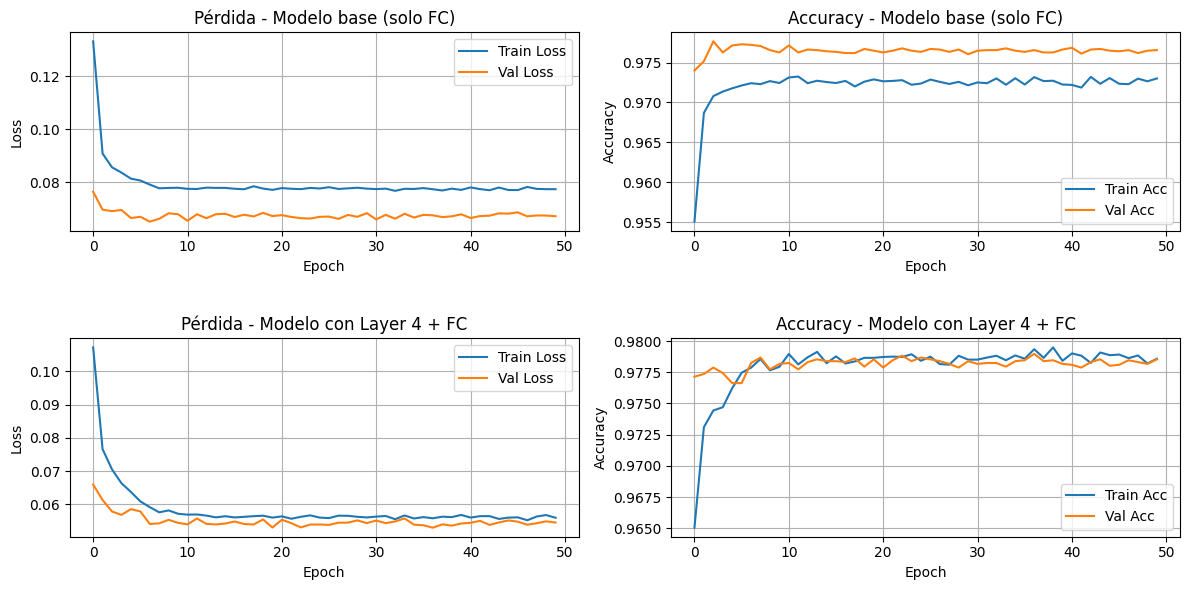
\includegraphics[scale=0.45]{doc_images/baseline.png}
		\caption{Modelos base. Curvas de pérdida (loss) y exactitud (accuracy) por época para dos configuraciones: un modelo que entrena solo la capa fully connected sobre una red base preentrenada congelada, y otro que también entrena la cuarta capa de dicha red.} 
		\label{fig:baseline}
	\end{figure}
\end{center}

\begin{center}
	\begin{figure}[H]
		\centering
		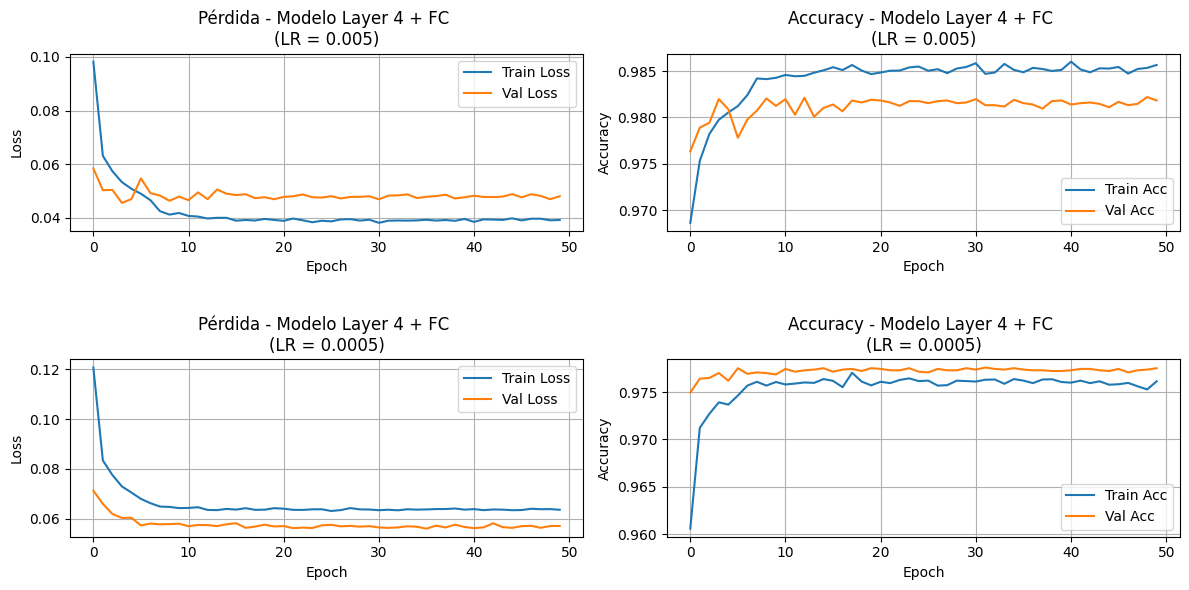
\includegraphics[scale=0.45]{doc_images/lr.png}
		\caption{Variación de tasa de aprendizaje. Curvas de pérdida (loss) y exactitud (accuracy) por época para dos configuraciones de tasa de aprendizaje: una con una tasa de 0.005 y otra con una tasa de 0.0005.} 
		\label{fig:lr}
	\end{figure}
\end{center}

\begin{center}
	\begin{figure}[H]
		\centering
		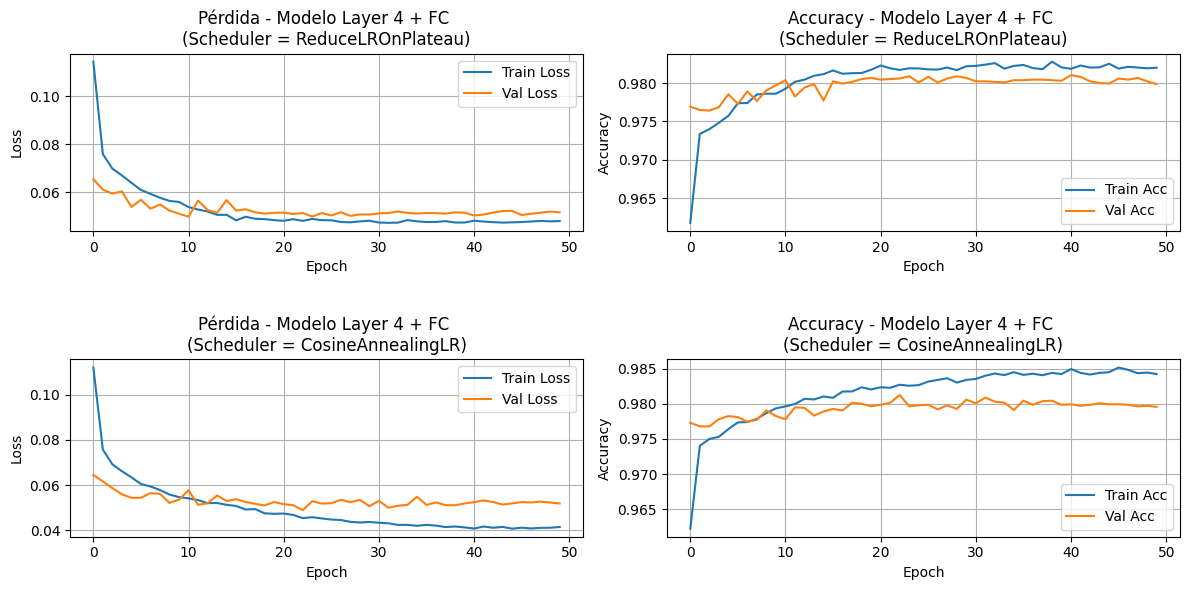
\includegraphics[scale=0.45]{doc_images/scheduler.png}
		\caption{Efecto de los schedulers. Curvas de pérdida (loss) y exactitud (accuracy) por época utilizando dos estrategias de programación de tasa de aprendizaje: ReduceLROnPlateau y CosineAnnealingLR.} 
		\label{fig:scheduler}
	\end{figure}
\end{center}

\begin{center}
	\begin{figure}[H]
		\centering
		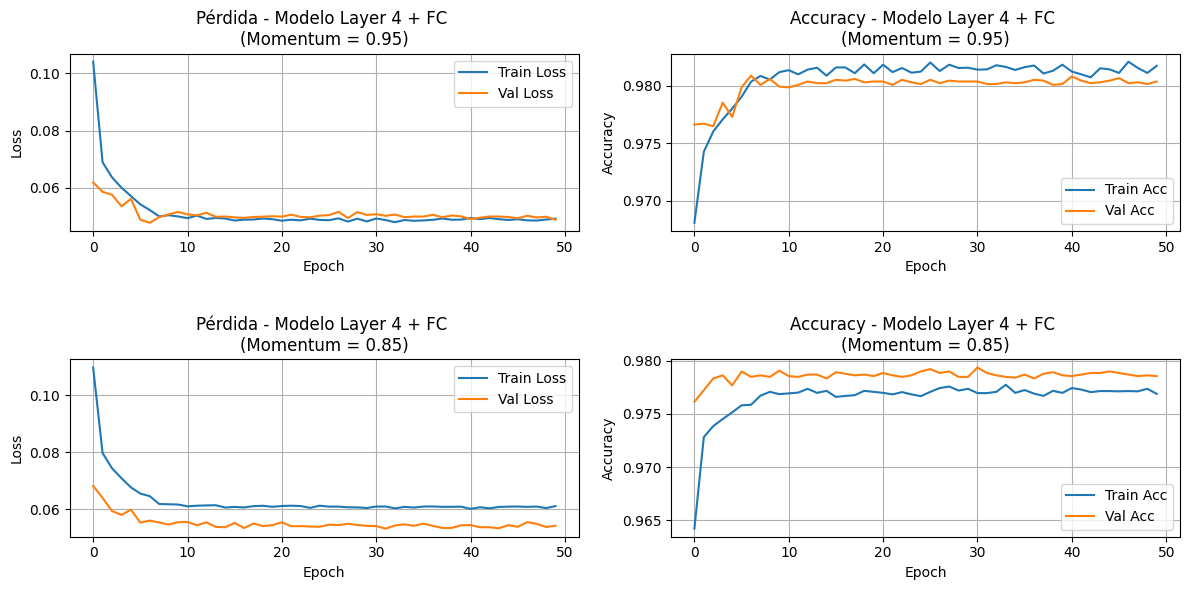
\includegraphics[scale=0.45]{doc_images/momentum.png}
		\caption{Efecto del Momentum. Curvas de pérdida (loss) y exactitud (accuracy) por época utilizando dos valores de momentum: 0.95 y 0.85.} 
		\label{fig:momentum}
	\end{figure}
\end{center}

\begin{center}
	\begin{figure}[H]
		\centering
		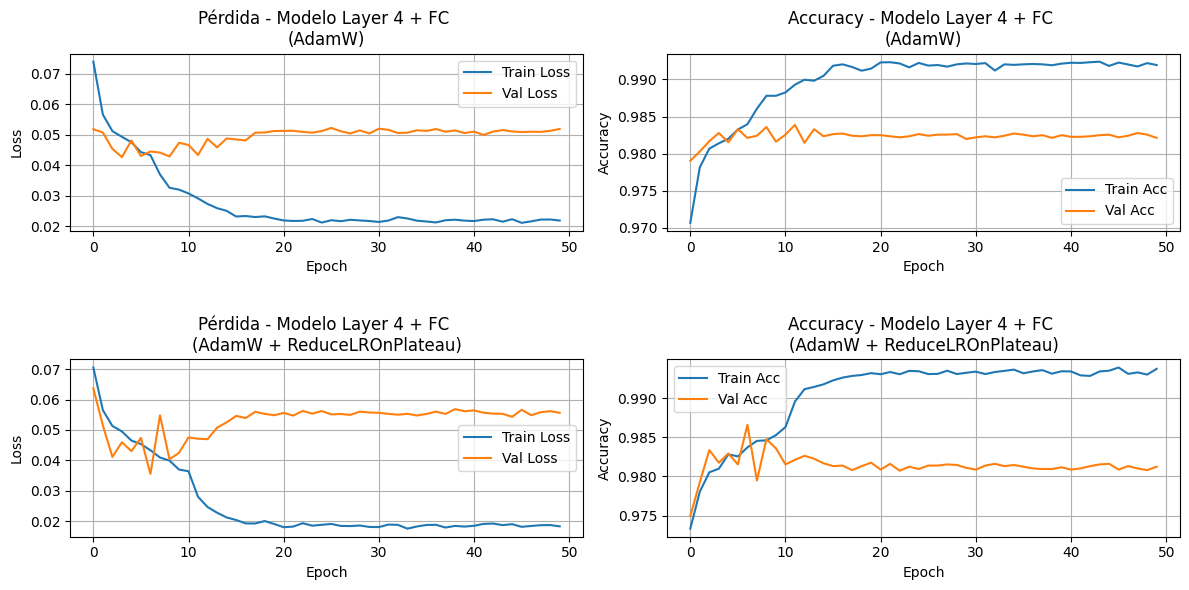
\includegraphics[scale=0.45]{doc_images/adam.png}
		\caption{Optimizador AdamW. Curvas de pérdida (loss) y exactitud (accuracy) por época para dos configuraciones basadas en AdamW: una utilizando únicamente AdamW, y otra combinada con ReduceLROnPlateau.} 
		\label{fig:adam}
	\end{figure}
\end{center}

\begin{center}
	\begin{figure}[H]
		\centering
		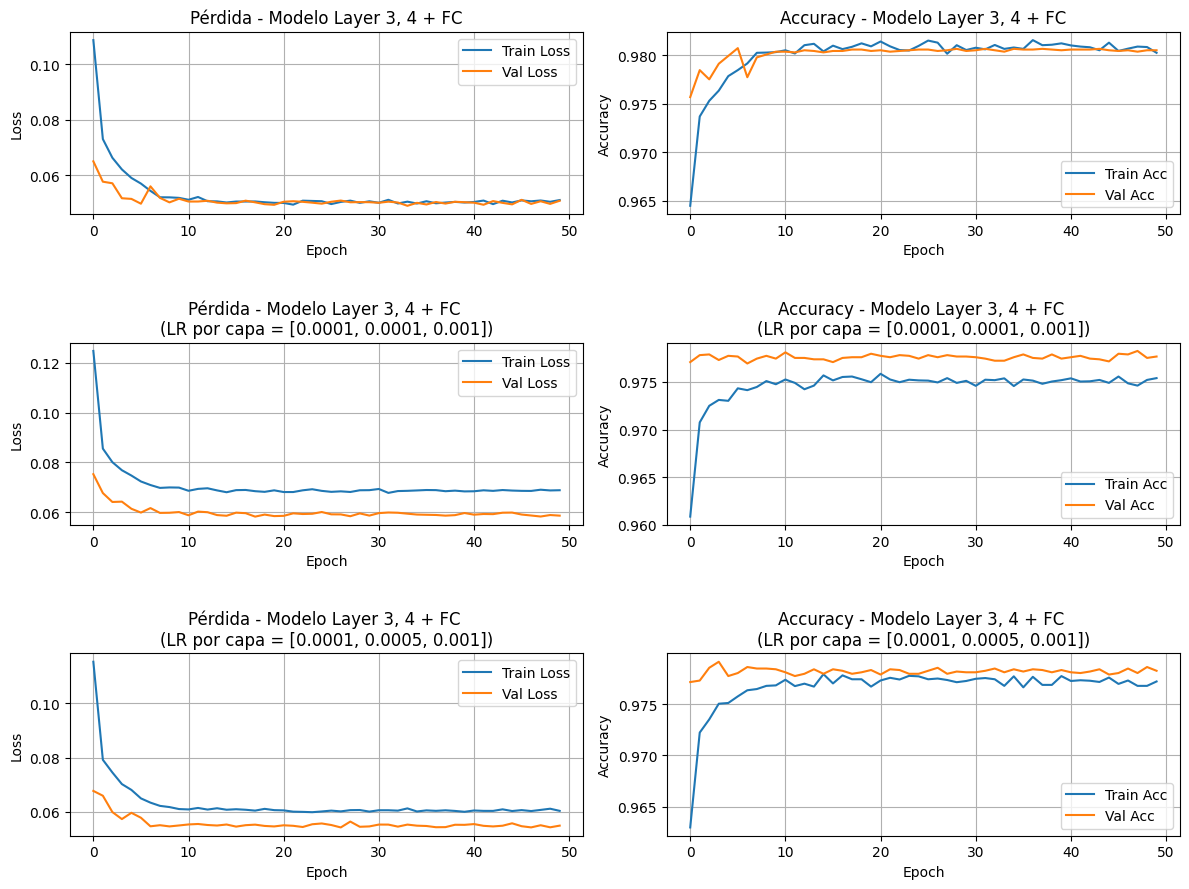
\includegraphics[scale=0.45]{doc_images/layer3.png}
		\caption{Descongelamiento de la capa 3. Curvas de pérdida y exactitud por época para tres configuraciones de fine-tuning de las capas 3 y 4 con distintas tasas de aprendizaje.} 
		\label{fig:layer3}
	\end{figure}
\end{center}

\begin{center}
	\begin{figure}[H]
		\centering
		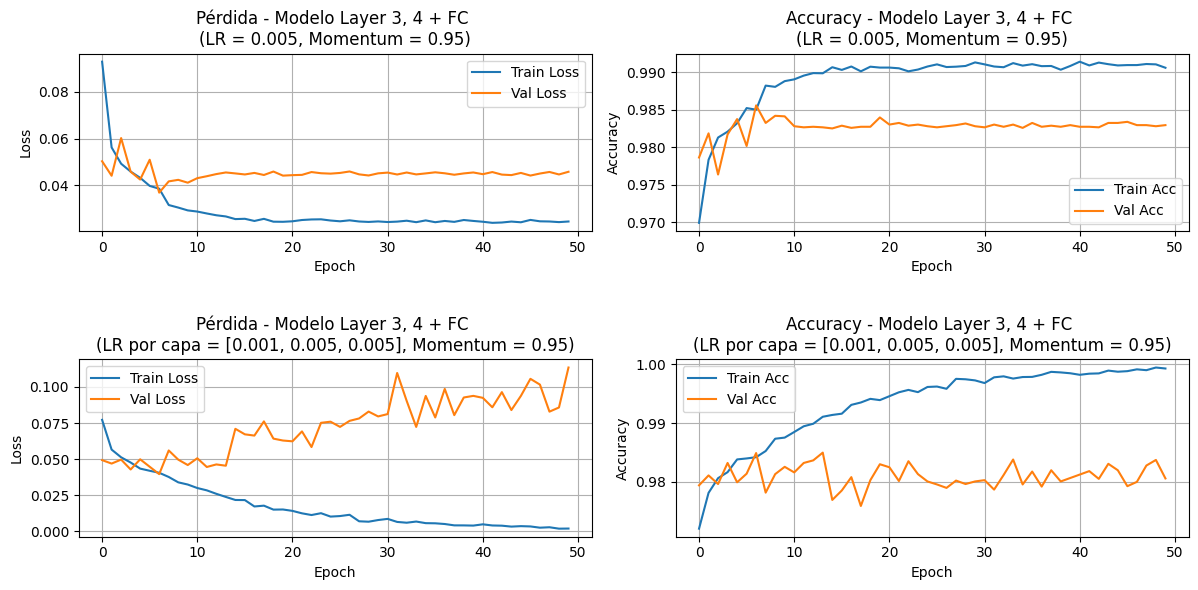
\includegraphics[scale=0.45]{doc_images/ultimas.png}
		\caption{Combinaciones de hiperparámetros. Curvas de pérdida y exactitud por época para dos configuraciones avanzadas de hiperparámetros: una combinando LR alta (0.005) con momentum 0.95, y otra empleando tasas de aprendizaje diferenciadas por capa ([0.001, 0.005, 0.005]) junto con momentum 0.95.} 
		\label{fig:ultimas}
	\end{figure}
\end{center}

La primera prueba, en la que se entrena únicamente la capa totalmente conectada (FC), ya muestra resultados positivos, lo que destaca el poder del transfer learning. A pesar de haber sido preentrenado en un conjunto de datos muy diferente al de imágenes de fondo de ojo, el modelo logra capturar representaciones que resultan útiles para esta nueva tarea. Esto demuestra que incluso con un ajuste mínimo, es posible obtener un desempeño aceptable, gracias a que las características aprendidas previamente son lo suficientemente generales como para transferirse a otros dominios.

Al permitir además el entrenamiento de la capa 4 (segunda prueba), se observa una mejora en el desempeño del modelo junto con una mejor capacidad de generalización (menor diferencia entre train y val). Esta mejora sugiere que, si bien las representaciones generales ya aportan una base sólida, afinar capas más profundas permite una mejor adaptación a las características específicas del nuevo conjunto de datos.

Las pruebas con diferentes tasas de aprendizaje muestran que, al darle mayor sinergia al proceso de aprendizaje, la loss converge más rápido y hay una mejora en el accuracy, pero también comienza a observarse algo de overfitting en los datos de entrenamiento.

En cuanto a los diferentes schedulers, tanto ReduceLROnPlateau como CosineAnnealingLR alcanzan valores similares de accuracy, aunque el segundo requiere más tiempo para completar el entrenamiento. Ninguno de los dos mejora el accuracy obtenido con un aumento de la learning rate. Sin embargo, a favor de ReduceLROnPlateau, se puede destacar que su comportamiento de convergencia es más suave y ayuda a reducir la diferencia entre las curvas de entrenamiento y validación, lo que indica una mejor capacidad de generalización.

La diferencia en el momentum de los modelos con SGD no mostró un impacto tan significativo como el logrado con el optimizador AdamW, el cual no solo mejora el accuracy, sino que, al combinarse con ReduceLROnPlateau, también mostró una convergencia más rápida y una tasa de error más baja en comparación con SGD.

Descongelar la capa 3 con distintas configuraciones de hiperparámetros no superó el rendimiento del modelo optimizado con AdamW, lo que sugiere que los mapas de características preentrenados en capas más profundas ya aportan la información necesaria para la tarea.

El modelo entrenado con AdamW y ReduceLROnPlateau alcanzó la mayor precisión de validación (98.66\% en la época 7), superando al resto de configuraciones. Aunque a partir de la época 10 muestra un incremento en la brecha entre entrenamiento y validación, indicativo de sobreajuste, su capacidad de converger rápidamente y el ajuste automático de la tasa de aprendizaje permiten aplicar early stopping en el punto óptimo. Por ello, y dado que el principal objetivo es maximizar la precisión en validación, el modelo final seleccionado para la fase de evaluación fue AdamW + ReduceLROnPlateau.

\section{Evaluación}
El cuadro \ref{tab:evaluacion} resume las métricas de desempeño obtenidas por el modelo final al ser evaluado sobre el conjunto de test. Se incluyen la precisión (precision), la sensibilidad (recall), el puntaje F1 (f1-score) y la cantidad de muestras por clase (support). Se observa que el modelo presenta un mayor rendimiento en la detección de imágenes de buena calidad, lo cual era esperable dado el desbalance de clases en el conjunto de entrenamiento. Consigue una precisión global del 97\%, lo que representa una reducción de aproximadamente 1,6 puntos porcentuales respecto al 98,6\% alcanzado durante el entrenamiento.

\begin{table}[H]
	\centering
	\renewcommand{\arraystretch}{1.5}
		\begin{tabular}{ ||ccccc||  }
			\hline
			\textbf{Clase} & \textbf{Precision} & \textbf{Recall} & \textbf{f1-score} & \textbf{Support} \\
			\hline
			0 (Buena) & 0.9775 & 0.9918 & 0.9846 & 46,317 \\
			\hline
			1 (Mala) & 0.7252 & 0.4884 & 0.5837 & 2,064 \\
			\hline
			Accuracy &  &  & 0.9703 & 48,381 \\
			\hline
			Macro promedio & 0.8514 & 0.7401 & 0.7841 & 48,381 \\
			\hline
			Promedio ponderado & 0.9668 & 0.9703 & 0.9675 & 48,381 \\
			\hline
		\end{tabular}
	\caption{Classification report del modelo ResNet-18 fine-tuned evaluado sobre test.}
	\label{tab:evaluacion}
\end{table}

El cuadro \ref{tab:matriz} presenta la matriz de confusión correspondiente al desempeño del modelo final sobre el conjunto de test. En ella se observa que el modelo clasifica correctamente 45,935 de las 46,317 imágenes de buena calidad (clase 0), mientras que identifica correctamente 1,008 de las 2,064 imágenes de mala calidad (clase 1). Sin embargo, se evidencia una mayor cantidad de falsos negativos (1,056), es decir, imágenes de mala calidad clasificadas erróneamente como buenas.

\begin{table}[H]
	\centering
	\renewcommand{\arraystretch}{1.5}
	\begin{tabular}{ ||lrr||  }
		\hline
		 & \textbf{Predicho: Buena (0)} & \textbf{Predicho: Mala (1)} \\
		\hline
		Real: Buena (0) & 45,935 & 382 \\
		\hline
		Real: Mala (1) & 1,056 & 1,008 \\
		\hline
	\end{tabular}
	\caption{Matriz de confusión del modelo ResNet-18 fine-tuned evaluado sobre test.}
	\label{tab:matriz}
\end{table}

Con el objetivo de interpretar las decisiones del modelo y analizar cuáles regiones de las imágenes fueron determinantes en la clasificación, se aplicó la técnica de visualización Grad-CAM \parencites{selvaraju2017gradcam}. Esta técnica permite identificar las zonas más relevantes para la predicción, superponiendo un mapa de activación sobre la imagen original.

\begin{center}
	\begin{figure}[H]
		\centering
		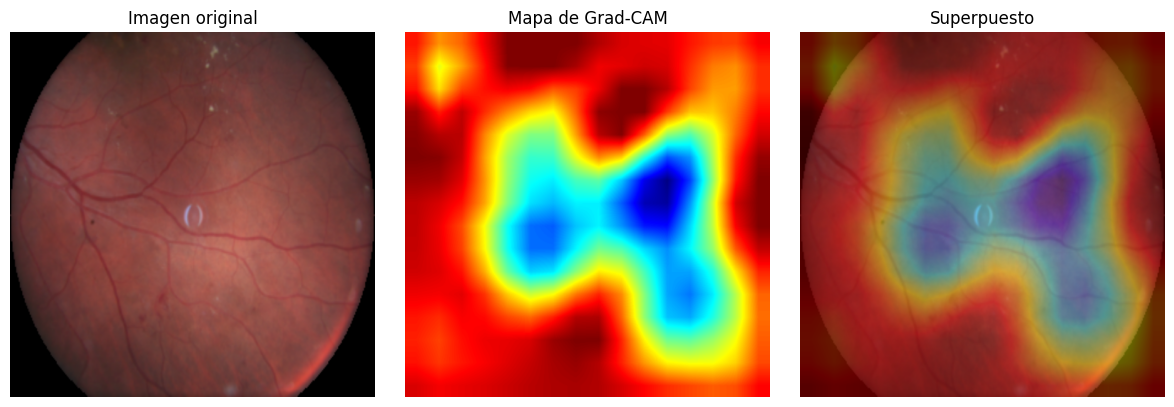
\includegraphics[scale=0.45]{doc_images/gram1.png}
		\caption{Visualización Grad-CAM de una imagen correctamente clasificada como de mala calidad.} 
		\label{fig:gram1}
	\end{figure}
\end{center}

En la Figura \ref{fig:gram1} se presenta un ejemplo correctamente clasificado como imagen de mala calidad, donde el modelo focaliza su atención en un reflejo generado por la cámara y en la ausencia de estructuras clave como el disco óptico y la mácula, indicadores consistentes con la etiqueta real.

\begin{center}
	\begin{figure}[H]
		\centering
		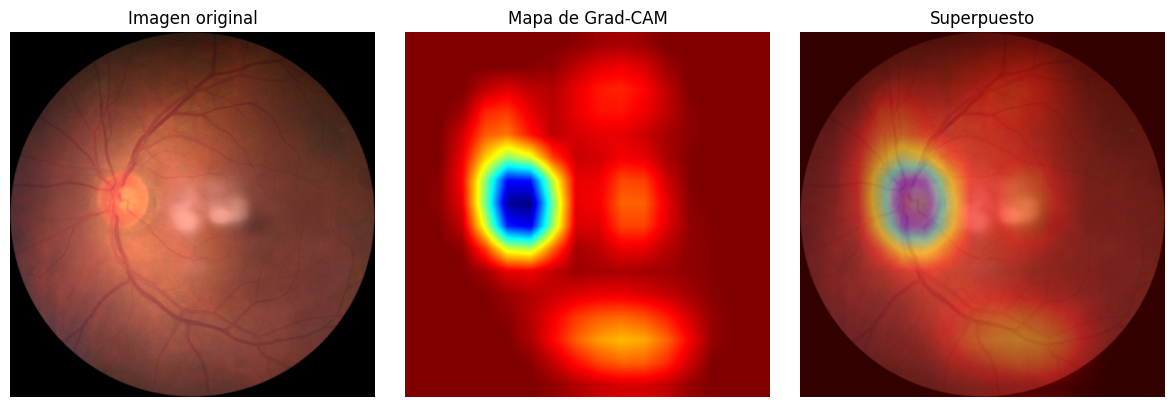
\includegraphics[scale=0.45]{doc_images/gram2.png}
		\caption{Visualización Grad-CAM de una imagen mal clasificada: el modelo la predice como de buena calidad, aunque está etiquetada como mala.} 
		\label{fig:gram2}
	\end{figure}
\end{center}

La Figura \ref{fig:gram2} muestra un caso mal clasificado, en el que la imagen es efectivamente de mala calidad, pero el modelo la predice como buena. Se observa que la atención se concentra en la mácula y los vasos sanguíneos visibles, lo que sugiere que el modelo prioriza la detección de ciertas estructuras anatómicas para inferir la calidad, incluso si existen artefactos en otras zonas.


\begin{center}
	\begin{figure}[H]
		\centering
		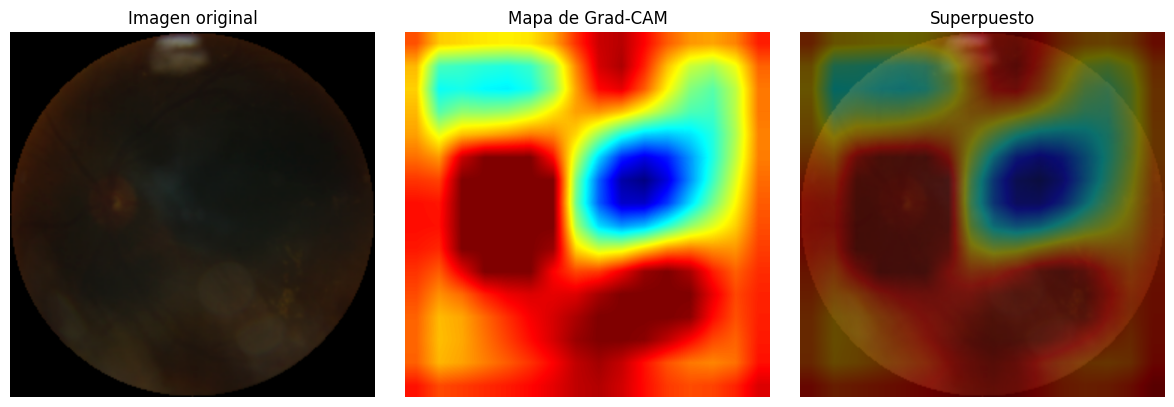
\includegraphics[scale=0.45]{doc_images/gram3.png}
		\caption{Visualización Grad-CAM de una imagen etiquetada como de buena calidad pero clasificada como de mala.} 
		\label{fig:gram3}
	\end{figure}
\end{center}

Finalmente, en la Figura \ref{fig:gram3} se presenta una imagen etiquetada como de buena calidad, pero clasificada por el modelo como de mala calidad. El modelo parece haber identificado correctamente que la imagen está oscura y contiene varios artefactos. Esto sugiere que, en algunos casos, la decisión del modelo podría incluso ser más coherente con criterios objetivos de calidad que la etiqueta asignada manualmente.

\section{Implementación y entorno de desarrollo}
La implementación del modelo se realizó en Python (3.10.15), utilizando el framework PyTorch (versión 2.5.0) para la definición, entrenamiento y evaluación de redes neuronales convolucionales. Se emplearon además las siguientes librerías complementarias: Torchvision (0.20.0) para la carga y transformación de imágenes, OpenCV (4.10.0) y PIL (10.4.0) para el procesamiento de imágenes, scikit-learn (1.5.2) para el cálculo de métricas de desempeño, NumPy (2.0.1) para operaciones matriciales, Matplotlib (3.9.2) para visualización de resultados, Pandas (2.2.3) para la manipulación de datos tabulares. El desarrollo se llevó a cabo en el entorno Visual Studio Code sobre un sistema operativo Windows 11 Pro. La ejecución del modelo se aceleró mediante una GPU NVIDIA GeForce RTX 4090 con 16 GB de memoria dedicada, utilizando CUDA versión 12.7 y el controlador NVIDIA 566.03. El equipo cuenta además con un procesador Intel Core (Intel64 Family 6 Model 186 Stepping 2) y 64 GB de memoria RAM. Todos los experimentos se realizaron en modo de usuario (WDDM), permitiendo la ejecución simultánea de procesos gráficos y de cómputo sin interferencias significativas en el rendimiento del modelo.

El código completo del modelo, así como los scripts utilizados para el entrenamiento, la evaluación y la generación de visualizaciones, se encuentra disponible en el siguiente repositorio: \url{https://github.com/gabimoran/MiM.git}
